%\documentclass{report}
%\usepackage[left=1.25in,right=1.25in,top=1in,bottom=1.5in]{geometry} % set different margins
\usepackage{placeins}
\usepackage{graphicx}
\usepackage{hyperref}
\usepackage{bookmark}
\usepackage{titlesec}
\usepackage[T1]{fontenc}
%\usepackage{amsmath}
\usepackage{tabularx}
\usepackage{ifpdf}
\usepackage{ae}
\usepackage{tikz}
\usepackage{colortbl}
\usepackage{caption}

\usepackage{wrapfig}
%\usepackage{../Packages/tikz-uml}% this package is for uml diagrams
\usepackage{Packages/tikz-uml}% this package is for uml diagrams
\usepackage{caption} % load caption package
\usepackage{enumitem}
\usepackage{listings}
\usepackage{amsmath}
\usepackage{subcaption}
\usepackage{xcolor}
\usepackage{listings}
\usepackage{tcolorbox}

\tcbuselibrary{listings}
\definecolor{LightGray}{gray}{0.95}
\usepackage{tcolorbox}
\definecolor{dkgreen}{RGB}{0,128,0}
\NewTotalTCBox{\commandbox}{ s v }
{verbatim,colupper=white,colback=black!75!white,colframe=black}
{\IfBooleanT{#1}{\textcolor{red}{\ttfamily\bfseries > }}%
\lstinline[language=command.com,keywordstyle=\color{blue!35!white}\bfseries]^#2^}
\lstset{ 
  backgroundcolor=\color{LightGray},
  basicstyle=\ttfamily,
  breaklines=true,
  captionpos=b,
  language=bash,
  frame=single
}


\tcbset{colframe=blue!50!black,colback=white,colupper=black,
fonttitle=\bfseries,nobeforeafter,center title}
\definecolor{mauve}{RGB}{224,176,255}

\usetikzlibrary{positioning}
\lstset{frame=tb,
  language=Python,
  aboveskip=3mm,
  belowskip=3mm,
  showstringspaces=false,
  columns=flexible,
  basicstyle={\small\ttfamily},
  numbers=none,
  numberstyle=\tiny\color{gray},
  keywordstyle=\color{blue},
  commentstyle=\color{dkgreen},
  stringstyle=\color{mauve},
  breaklines=true,
  breakatwhitespace=true,
  tabsize=3
}
\setcounter{secnumdepth}{4}
\setcounter{tocdepth}{4}
\addcontentsline{toc}{section}{Introduction}

\renewcommand{\thesection}{\Roman{section}} 
\renewcommand{\thesubsection}{\arabic{subsection}}
\titlespacing{\subsection}{5pt}{1em}{0pt}
\graphicspath{ {./Ilustrations}{./}{./images}}
%\graphicspath{ {../Ilustrations}{../images}}

\tikzstyle{usecase}=[ellipse, fill=white, draw=black, thick, inner sep=2pt, text centered]
%\begin{document}
\chapter{Project Framework and Methodology}
\section*{Introduction}
 %Presentation of the  enterprise
\section{Presentation of the  enterprise}
esca Group is a family-run company with a background in textiles that has successfully ventured into the automotive industry, specifically automotive seating. Emulating the approach of a French automotive manufacturing house, Tesca Group meticulously crafts each piece, from its atelier to its global production sites. The company strives to embody the same creative audacity and prides itself on being a partner to major automotive manufacturers like : 



\begin{figure}[htbp]
\centering
\begin{subfigure}{0.16\textwidth}
  \centering
  \includegraphics[width=\linewidth]{ALPINE}
\end{subfigure}%
\begin{subfigure}{0.16\textwidth}
  \centering
  \includegraphics[width=\linewidth]{AUDI}
\end{subfigure}%
\begin{subfigure}{0.16\textwidth}
  \centering
  \includegraphics[width=\linewidth]{bentley-1}
\end{subfigure}%
\begin{subfigure}{0.16\textwidth}
  \centering
  \includegraphics[width=\linewidth]{BMW-1}
\end{subfigure}%
\begin{subfigure}{0.16\textwidth}
  \centering
  \includegraphics[width=\linewidth]{NISSAN}
\end{subfigure}%
\begin{subfigure}{0.16\textwidth}
  \centering
  \includegraphics[width=\linewidth]{CITROEN}
\end{subfigure}

\vspace{10pt} % adjust the vertical spacing between rows

\begin{subfigure}{0.16\textwidth}
  \centering
  \includegraphics[width=\linewidth]{CUPRA-1}
\end{subfigure}%
\begin{subfigure}{0.16\textwidth}
  \centering
  \includegraphics[width=\linewidth]{DACIA}
\end{subfigure}%
\begin{subfigure}{0.16\textwidth}
  \centering
  \includegraphics[width=\linewidth]{DS}
\end{subfigure}%
\begin{subfigure}{0.16\textwidth}
  \centering
  \includegraphics[width=\linewidth]{FAW}
\end{subfigure}%
\begin{subfigure}{0.16\textwidth}
  \centering
  \includegraphics[width=\linewidth]{FORD}
\end{subfigure}%
\begin{subfigure}{0.16\textwidth}
  \centering
  \includegraphics[width=\linewidth]{HYUNDAI}
\end{subfigure}

\caption{Tesca's partners}
\end{figure}





With a clientele consisting of demanding visionaries who shape the future of mobility, Tesca Group positions itself as a reliable and flexible partner, accompanying its clients in their pursuit of innovation and competitiveness. The company believes that adopting a long-term and eco-friendly vision is crucial for sustainable growth, constantly pushing for excellence rather than settling for mediocrity.

Sustainability is a concrete and integral part of Tesca Group's approach. The company is committed to sustainable development and actively incorporates environmental and social values into its products, services, and activities within the automotive industry. Since 2004, Tesca Group has been dedicated to controlling its ecological footprint, and the executive management maintains and expands upon these efforts. The company adheres to the values and principles of the Global Compact through its Ethics Charter, with the objective of obtaining ISO 14001 certification for all its sites.

Tesca Group's environmental policy revolves around five major directions: behaving in an environmentally responsible manner, optimizing and controlling industrial waste, optimizing energy consumption and natural resources, participating in the reduction of the ecological footprint throughout the design and production processes, and ensuring compliance with environmental regulations and requirements.

Innovation is a driving force within Tesca Group, with a constant emphasis on generating new ideas and executing them effectively. The company's research programs focus on key themes in the automotive industry, such as weight reduction, optimized part design, and ecological footprint expertise, while prioritizing user comfort, functionality, and safety. Tesca Group holds numerous patents in the conception, design, and manufacturing of automotive parts and seat components, including headrests, armrests, upholstery, padding, and "smart textiles."

Industrial excellence is a cornerstone of Tesca Group's strategy, whether through its local production sites or research centers. The company strives to provide reliable processes that meet the evolving market expectations worldwide. Tesca Group empowers its teams through a culture of continuous improvement, with competitiveness, efficiency, and exceptional service forming the foundation of its industrial success. SPRINT (Tesca's INdustrial Production System) is employed to engage collaborators at all levels, aiming to standardize procedures and ensure perpetual progress in industrial performance. Shared values among Tesca Group employees include excellence, self-discipline, commitment, autonomy, and pragmatism.

Tesca Group's Quality policy aligns with five major directions: meeting commitments to conformity, cost, and deadlines; aligning industrial and purchasing performance with the highest quality criteria; standardizing existing processes to offer innovative products; prioritizing process control and prevention; and continuously enhancing the skills of its teams.

In terms of its history, Tesca Group has a notable timeline of achievements. Starting in 1960 with the provision of Citroën 2CV roofs, the company went on to pioneer and apply the Foam In Place technology in 1978. In 1983, Tesca Group established its Design Studio in Paris, followed by the creation of the CERA research and development center in Reims in 1993. By the year 2000, the company had expanded its production capabilities worldwide. In 2016, Tesca Group underwent a significant transformation, becoming Trèves TSC.

Overall, Tesca Group has established itself as a reputable partner to major automotive manufacturers, driven by a commitment to sustainability, innovation, industrial excellence, and quality. Through its diverse range of products and services, the company aims to shape the future
\subsection{description of the  enterprise }
\subsection{description of the  enterprise's services}
\subsection{administrative organization chart of the enterprise}
\vspace{1em}
 %Presentation of the  enterprise
\section{Study of the existing system}
\subsection{description of the existing system }
\subsection{criticism of the existing system}
\subsection{administrative organization chart of the enterprise}
\vspace{1em}
 %Working methodology and modeling language
\section{Working methodology and modeling language}
\subsection{Traditional work methodology vs Agile method }
In order to ensure a successful outcome for an IT project, it is crucial to follow a structured work methodology throughout its entire lifecycle. A work methodology provides a framework for project management, which includes defining tasks, assigning responsibilities, monitoring progress, and ensuring that deadlines are met.\cite{PGC10}


\vspace{0.25cm}
There are many different methodologies that can be used for IT project management, such as Agile\cite{Aw15} and Heavyweight\cite{Aw15} . Each methodology has its own set of principles, practices, and tools that are designed to optimize project performance and efficiency.

\FloatBarrier
\begin{table}[h]

\centering
\tcbox[
  left=0mm,
  right=0mm,
  top=0mm,
  bottom=0mm,
  boxsep=0mm,
  toptitle=0.5mm,
  bottomtitle=0.5mm, title = Comparison of heavyweight and agile methods \cite{PGC10}]{%
\arrayrulecolor{blue!50!black}\renewcommand{\arraystretch}{1.2}%



\begin{tabular}{|l|c|r|}
\hline
\multicolumn{1}{|l|}{         } & \multicolumn{1}{|c|}{Heavyweight Methods}& \multicolumn{1}{|c|}{Agile Methods} \\
\hline
Approach & Adaptive  & Predictive  \\
\hline
Success Measurement & Business Value & Conformation to plan \\
\hline
Project size & Small & Large \\
\hline
Management Style & Decentralized & Autocratic \\
\hline
Perspective to Change & Change Adaptability & Change Sustainability \\
\hline
Culture & Leadership-Collaboration & Command-Control \\
\hline
Documentation & Low & Heavy \\
\hline
Emphasis & People-Oriented & Process-Oriented \\
\hline
Cycles & Numerous & Limited \\
\hline
Domain & Unpredictable/Exploratory & Predictable \\
\hline
Upfront Planning & Minimal & Comprehensive \\
\hline
Return on Investment & Early in Project & End of Project \\
\hline
Team Size & Small/Creative & Large \\
\hline
\end{tabular}}
    \addcontentsline{lot}{table}{Comparison of heavyweight and agile methods \cite{PGC10}}

\label{table:comparison}
\end{table}
\FloatBarrier

\newpage
\subsection{Chosen methodology: SCRUM}
\FloatBarrier
\begin{figure}[h]
         \centering
        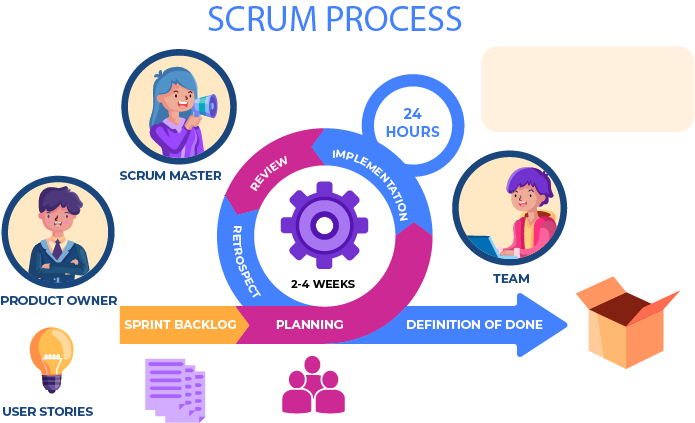
\includegraphics[width=0.6\textwidth]{SCRUM PROCESS}
   
        \caption{Scrum process}
        \label{fig:Scrum process}
    \end{figure}
\FloatBarrier
   
\subsubsection{Reasons}
The adopted development methodology is Scrum. The choice is based on Scrum's strengths, which can be summarized as follows:
\begin{itemize}
\item \textbf{Flexibility} : Scrum is designed to be flexible and adaptable to changing project requirements. This allows teams to respond quickly to changes in the project environment.\cite{Aw15}\cite{PGC10}

\item \textbf{Collaboration}: Scrum emphasizes collaboration and communication between team members. \cite{Aw15}\cite{PGC10}

\item \textbf{Continuous Improvement} : Scrum includes regular reviews and retrospectives, which provide opportunities for the team to reflect on their progress and identify areas for improvement.\cite{Aw15}\cite{PGC10}

\item \textbf{Transparency} : Scrum provides a framework for making project progress and status visible to all stakeholders.\cite{Aw15}\cite{PGC10}

\item \textbf{Empowerment}: Scrum encourages team members to take ownership of their work and make decisions independently.\cite{Aw15}\cite{PGC10}
\end{itemize}
\subsubsection{The Scrum team}
And we can not end this section without talking about the scrum team  which is composed of:
\begin{itemize}

\item The \textbf{Scrum Master} is responsible for implementing and maximizing the benefits of the Scrum process. They facilitate Scrum events, remove obstacles, and promote continuous improvement.\cite{PGC10}
\item The \textbf{team} is a cross-functional group of self-motivated individuals who share tasks and responsibilities, working collaboratively to manage themselves and deliver successful product increments every Sprint.\cite{PGC10}
\item The \textbf{Product Owner} is typically the project's key stakeholder, who has a deep understanding of users, the marketplace, competitors, and trends. They are responsible for managing the Product Backlog to maximize the project's value and representing the interests of everyone with a stake in the project and its resulting product.\cite{PGC10}
\end{itemize}
\subsubsection{Other terminologies}
Let's now look at some options specific to the agile mode and more particularly to SCRUM.
\begin{itemize}
\item A \textbf{sprint} is a time-boxed period when a SCRUM team works to complete a set amount of work in one repeating cycle, typically lasting no longer than one month and fixed throughout the overall work.\cite{PGC10}
\item The \textbf{Product Backlog}   in SCRUM is a prioritized list of items (or user stories) that represent work needed to deliver a product or service, including estimated completion times. It changes with business conditions or technology.\cite{PGC10}
\item Th\textbf{User stories} are often used to describe the Product Backlog items in terms of their value to the end user of the product.\cite{PGC10}
\end{itemize}
\subsection{Modeling languages : UML and SysMl}
\subsubsection{UML}

\textbf{UML} , or Unified Modeling Language, is a standardized visual language for describing software systems composed of a set of diagrams, each of which provides a different view of the project to be addressed.\cite{HMB03}

\textbf{UML}  provides us with diagrams to represent the system to be developed: its operation, startup, actions that can be performed by the system, etc. Creating these diagrams is therefore equivalent to modeling the needs of the software to be developed.\cite{HMB03}

\begin{itemize}
\item Structure diagrams 
\begin{itemize}
\item Class Diagram
\item Component Diagram
\item Deployment Diagram
\item Object Diagram
\item Package Diagram
\item Profile Diagram
\item Composite Structure Diagram
\end{itemize}
\item Behavioral Diagrams
\begin{itemize}
\item Use Case Diagram
\item Activity Diagram
\item State Machine Diagram
\item Sequence Diagram
\item Communication Diagram
\item Interaction Overview Diagram
\item Timing Diagram
\end{itemize}
\end{itemize}

\subsubsection{SysMl}
\textbf{SysMl},  or Systems Modeling Language, is a graphical language used by MBSE (Model-Based Systems Engineering) practitioners to create system models and communicate ideas about system designs to stakeholders. It is a language that has a grammar and vocabulary consisting of graphical notations that have specific meanings. The purpose of SysML is to visualize and communicate a system's design among stakeholders.\cite{LD13}

The grammar and notations of SysML are defined in a standards specification published by the Object Management Group, which is a consortium of computer industry companies, government agencies, and academic institutions. SysML is an extension of a subset of the Unified Modeling Language (UML), and its complete definition requires referring to parts of the UML specification document as well.\cite{LD13}
\begin{itemize}
\item Behavior diagrams\cite{LD13}
\begin{itemize}
\item Activity diagram
\item State machine diagram
\item Sequence diagram
\item Use case diagram
\item Communication diagram
\end{itemize}
\item Structure diagrams\cite{LD13}
\begin{itemize}
\item Block definition diagram
\item Internal block diagram
\item Parametric diagram
\item Package diagram
\item Composite structure diagram
\end{itemize}
\item Requirement diagram\cite{LD13}
\end{itemize}
\vspace{1em}

\section{Project management with SCRUM }
\subsection{Team and roles}
\FloatBarrier
\begin{table}[h]

\centering
\tcbox[
  left=0mm,
  right=0mm,
  top=0mm,
  bottom=0mm,
  boxsep=0mm,
  toptitle=0.5mm,
  bottomtitle=0.5mm, title = SCRUM Actors]{%
\arrayrulecolor{blue!50!black}\renewcommand{\arraystretch}{1.2}%



 \begin{tabular}{|l|l|p{9cm}|}
    \hline
    % after \\: \hline or \cline{col1-col2} \cline{col3-col4} ...
    Role & Actor & Mission \\
    \hline
    Team & Ahmed Omrani &Conception, development, unit testing, deployment. \\
    \hline
    SCRUM master & Radhwen Aloui &Ensure the smooth running of the SCRUM methodology.. \\
    \hline
    Product owner & ********** &Define the product features and ensure their conformity. \\
    \hline
  \end{tabular}}
    \addcontentsline{lot}{table}{SCRUM Actors}

\label{ActScrum}
\end{table}

\FloatBarrier


\subsection{Backlog Product}
\vspace{1em}
\section*{Conclusion}
%\begin{thebibliography}{9}
%\bibitem{Aw15}M. A. Awad, 2015. \emph{A Comparison between Agile and Traditional Software Development Methodologies 
%}.

%\bibitem{PGC10}Pete Deemer, Gabrielle Benefield, Craig Larman, Bas Vodde, 2010. \emph{THE
%SCRUM PRIMER}.
%\bibitem{HMB03}Hans-Erik Eriksson, Magnus Penker, Brian Lyons
%, 2003. \emph{UML 2 toolkit}.
%\bibitem{LD13}Lenny Delligatti , 2013. \emph{SysML Distilled A Brief Guide}.
%\bibitem{MA18} Mohamed FEZARI and Ali Al Dahoud, 2018. \emph{Integrated Development Environment “IDE” For Arduino}.
%\bibitem{BMIPC17}Bernadette M. Randles, Milena S. Golshan, Irene V. Pasquetto and Christine L. Borgman, 2017. \emph{Using the Jupyter Notebook as a Tool for Open Science: An Empirical Study}.
%\bibitem{SD20}Slobodan Dmitrović, 2020. \emph{ Modern C++ for Absolute Beginners: A Friendly Introduction to C++ Programming Language and C++11 to C++20 Standards}.
%\bibitem{CD21}Chakraborty D.,2021. \emph{ OpenCV Contour Approximation ( cv2.approxPolyDP ),}.
%\bibitem{WG10}Willow Garage, 2010. \emph{OpenCV Reference Manual v2.2}.






%\end{thebibliography}




%\end{document}